\documentclass{standalone}
\usepackage[latin1]{inputenc}
\usepackage{tikz}
\usetikzlibrary{automata,positioning, arrows}
\tikzset{->, 
>=stealth, node distance=10cm,every state/.style={thick,scale=3,fill=gray!10}, % sets the properties for each ’state’ node
initial text=$ $, % sets the text that appears on the start arrow
%every edge/.style = {font=\large}
}
\begin{document}
%    \begin{figure}
    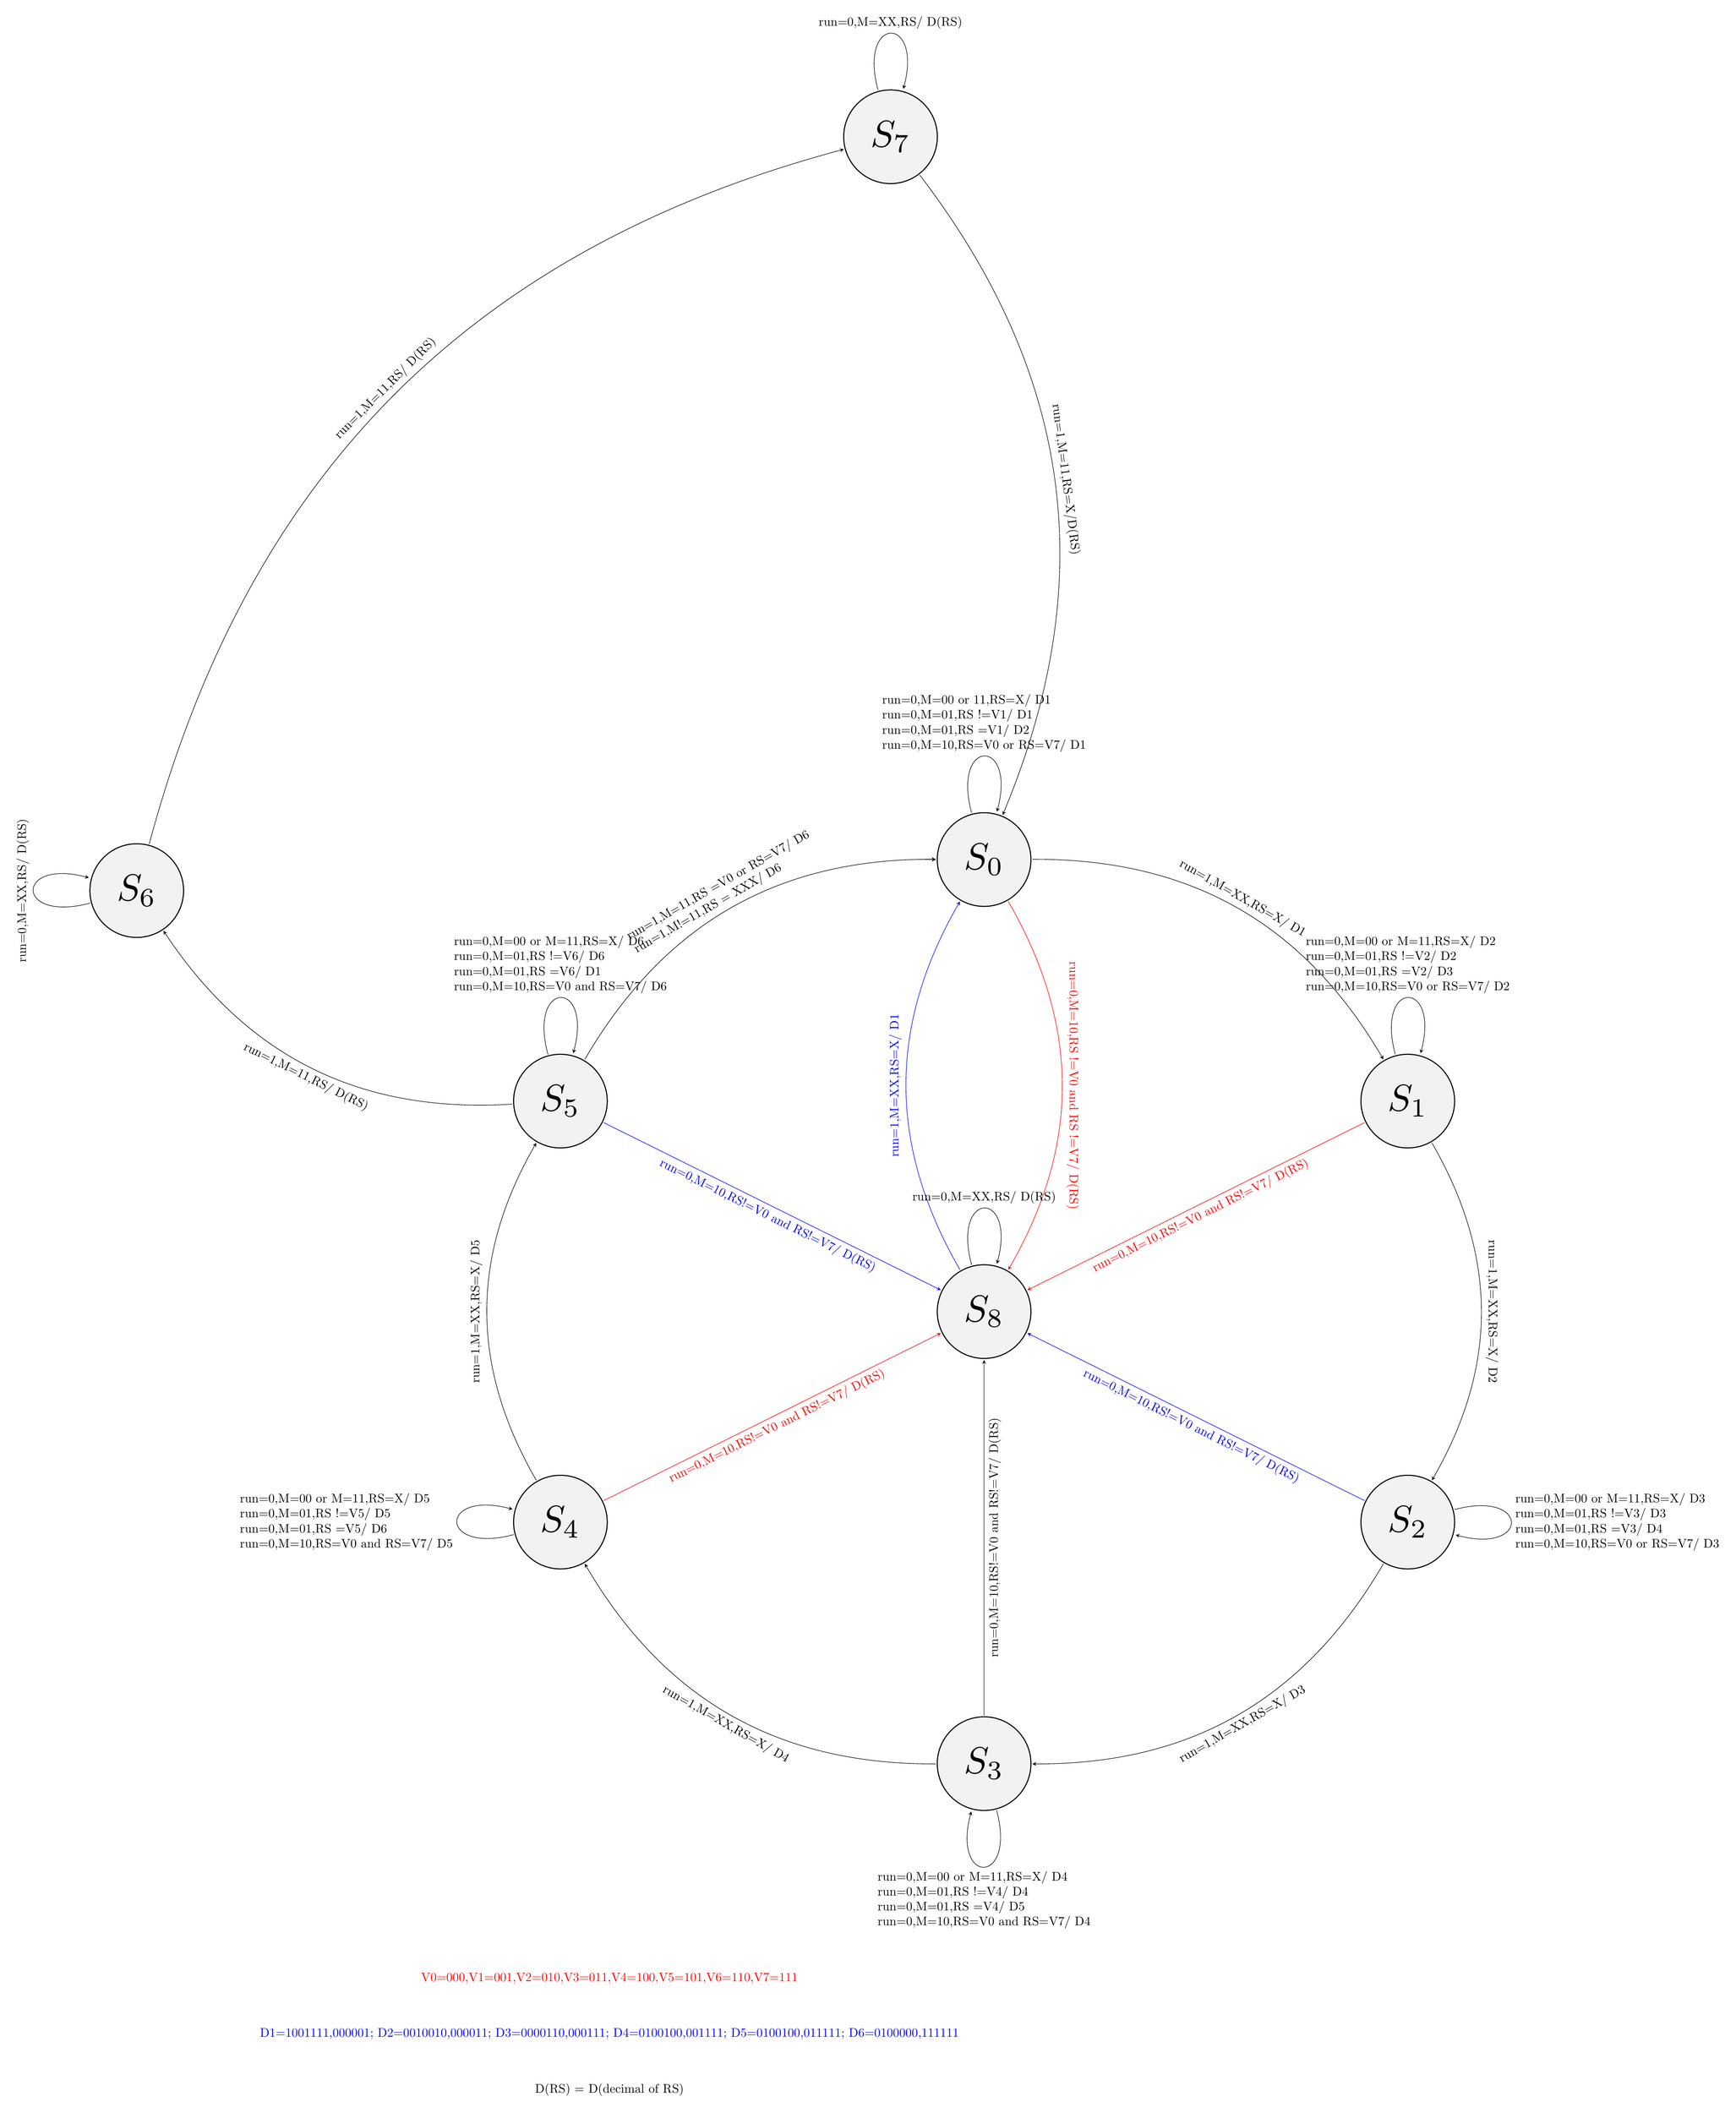
\begin{tikzpicture}
    \node[state,align=center] (S8) {$S_8$};
    \node[state,initial,above= of S8,align=center] (S0) {$S_0$};
    \node[state,above right= 4cm and 10cm  of S8,align=center] (S1) {$S_1$};
    \node[state,below right = 4cm and 10cm of S8,align=center] (S2) {$S_2$};
    \node[state,below = 10cm of S8,align=center] (S3) {$S_3$};
    \node[state,below left = 4cm and 10cm of S8,align=center] (S4) {$S_4$};
    \node[state,above left =4cm and 10cm of S8,align=center] (S5) {$S_5$};
    \node[state,above left =4cm and 10cm of S5,align=center] (S6) {$S_6$};
    \node[state,above right of=S6,align=center] (S7) {$S_7$};

    \draw (S0) edge[bend left,above] node [above,sloped,align=left]{ run=1,M=XX,RS=X/ D1} (S1)
          (S0) edge[red,bend left,above] node [above,sloped,align=left]{run=0,M=10,RS !=V0 and RS !=V7/ D(RS)} (S8)
          (S0) edge[loop above] node [above,sloped,align=left]{ run=0,M=00 or 11,RS=X/ D1 \\run=0,M=01,RS !=V1/ D1 \\run=0,M=01,RS =V1/ D2 \\ run=0,M=10,RS=V0 or RS=V7/ D1 } (S0)
          (S1) edge[bend left,above] node [above,sloped,align=left]{ run=1,M=XX,RS=X/ D2} (S2)
          (S1) edge[red,left,above] node [below,sloped,align=left]{run=0,M=10,RS!=V0 and RS!=V7/ D(RS)} (S8)
          (S1) edge[loop above] node [align=left]{ run=0,M=00 or M=11,RS=X/ D2 \\run=0,M=01,RS !=V2/ D2 \\run=0,M=01,RS =V2/ D3\\ run=0,M=10,RS=V0 or RS=V7/ D2 } (S1)
          (S2) edge[bend left,above] node [below,sloped,align=left]{ run=1,M=XX,RS=X/ D3} (S3)
          (S2) edge[blue,left,above] node [below,sloped,align=left]{run=0,M=10,RS!=V0 and RS!=V7/ D(RS)} (S8)
          (S2) edge[loop right] node [align=left]{ run=0,M=00 or M=11,RS=X/ D3 \\run=0,M=01,RS !=V3/ D3 \\run=0,M=01,RS =V3/ D4\\ run=0,M=10,RS=V0 or RS=V7/ D3 } (S2)
          (S3) edge[bend left,above] node [below,sloped,align=left]{ run=1,M=XX,RS=X/ D4} (S4)
          (S3) edge[black,left,above] node [below,sloped,align=left]{run=0,M=10,RS!=V0 and RS!=V7/ D(RS)} (S8)
          (S3) edge[loop below]  node [below,sloped,align=left](S3Loop){ run=0,M=00 or M=11,RS=X/ D4\\run=0,M=01,RS !=V4/ D4 \\run=0,M=01,RS =V4/ D5\\ run=0,M=10,RS=V0 and RS=V7/ D4 } (S3)
          (S4) edge[bend left,above] node [above,sloped,align=left]{ run=1,M=XX,RS=X/ D5} (S5)
          (S4) edge[red,left,above] node [below,sloped,align=left]{run=0,M=10,RS!=V0 and RS!=V7/ D(RS)} (S8)
          (S4) edge[loop left] node [align=left]{ run=0,M=00 or M=11,RS=X/ D5 \\run=0,M=01,RS !=V5/ D5 \\run=0,M=01,RS =V5/ D6\\ run=0,M=10,RS=V0 and RS=V7/ D5 } (S4)
          (S5) edge[bend left,above] node[above,sloped,align=left]{run=1,M=11,RS =V0 or RS=V7/ D6 \\ run=1,M!=11,RS = XXX/ D6} (S0)
          (S5) edge[loop above] node [above,sloped,align=left]{ run=0,M=00 or M=11,RS=X/ D6\\run=0,M=01,RS !=V6/ D6 \\run=0,M=01,RS =V6/ D1\\ run=0,M=10,RS=V0 and RS=V7/ D6 } (S5)
          (S5) edge[bend left,above] node [below,sloped,align=left]{ run=1,M=11,RS/ D(RS)  } (S6)
          (S5) edge[blue,left,above] node [below,sloped,align=left]{run=0,M=10,RS!=V0 and RS!=V7/ D(RS)} (S8)
          (S6) edge[bend left,above] node[above,sloped,align=left]{ run=1,M=11,RS/ D(RS)  } (S7)
          (S7) edge[bend left,above]  node[above,sloped,align=left]{ run=1,M=11,RS=X/D(RS)  }(S0)
          (S8) edge[blue,bend left,above] node [above,sloped,align=left]{run=1,M=XX,RS=X/ D1} (S0)
          (S6) edge[loop left] node [above,sloped,align=left]{ run=0,M=XX,RS/ D(RS)} (S6)
          (S7) edge[loop above] node [above,sloped,align=left]{ run=0,M=XX,RS/ D(RS)} (S7)
          (S8) edge[loop above] node [above,align=left]{ run=0,M=XX,RS/ D(RS)} (S8);

        \node[red,below left = 1cm and 2cm of S3Loop] (Legend1)  {V0=000,V1=001,V2=010,V3=011,V4=100,V5=101,V6=110,V7=111};
        \node[blue,below= 1cm of Legend1] (Legend2) {D1=1001111,000001; D2=0010010,000011; D3=0000110,000111; D4=0100100,001111; D5=0100100,011111; D6=0100000,111111 };
        \node[black,below= 1cm of Legend2] {D(RS) = D(decimal of RS)};
    \end{tikzpicture}
%    \caption {FSM diagram of 3 bit sequence detector}
%    \label {Fig.1} 
%   \end{figure}
\end{document}
